%%
%% 2April2008.tex
%% 
%% Made by Alex Nelson
%% Login   <alex@tomato>
%% 
%% Started on  Wed Dec 17 15:47:14 2008 Alex Nelson
%% Last update Wed Dec 17 15:47:14 2008 Alex Nelson
%%

Remember Euler's formula
\begin{equation}
e^{i\theta} = \cos(\theta)+i\sin(\theta).
\end{equation}
Observe that
\begin{equation}
e^{-i\theta}=e^{i(-\theta)} = \cos(-\theta)+i\sin(-\theta)
\end{equation}
and
\begin{equation}
\overline{e^{i\theta}}=e^{-i\theta} =
\cos(\theta)-i\sin(\theta).
\end{equation}
We set $e^{-i\theta}=e^{-i\theta}$ and find from the real
part
\begin{equation}
\cos(-\theta)=\cos(\theta)
\end{equation}
and from the imaginary part
\begin{equation}
\sin(-\theta)=-\sin(\theta).
\end{equation}
We call $\cos(\theta)\approx 1-\theta^2/2+...$ an \textbf{even function} and
$\sin(\theta)\approx \theta-\theta^3/6+...$ an \textbf{odd function}. 

\begin{defn}
Let $f:\mathbb{R}\to\mathbb{R}$ be a function, then $f$ is
\textbf{periodic with period $p$} (or $p$-\textbf{periodic})
if
\begin{equation}
f(x+p)=f(x)
\end{equation}
holds.
\end{defn}

\begin{ex}
The functions $\cos(\theta)$, $\sin(\theta)$ and
$\exp(i\theta)$ are all $2\pi$-periodic.
\end{ex}

\begin{lem}
If we have a $p$-periodic function $f$, then
\begin{equation}
\int^{a+p}_{a}f(x)dx
\end{equation}
is independent of $a$.
\end{lem}
\begin{proof}
If we change $a$ by some $c$ (so $a\to a+c$) then
\begin{subequations}
\begin{align}
\int^{a+c+p}_{a+c}f(x)dx &= \int^{a+p}_{a+c}f(x)dx +
\int^{a+c+p}_{a+p}f(x)dx\quad(\text{by linearity of integral})\\
&= \int^{a+p}_{a+c}f(x)dx +
\int^{a+c}_{a}f(x)dx\quad(\text{by periodicity of $f(x)$}) \\
&= \int^{a+p}_{a}f(x)dx\quad(\text{collecting terms})
\end{align}
\end{subequations}
where we justify the second step (the one justified in a
handwavy way with the ``periodicity of $f$'') by using the
Riemann sum and noting such reasoning works for that
particular definition of the integral and we use it here too.
\end{proof}

\begin{defn}
Let $f:\mathbb{R}\to\mathbb{R}$ be $2\pi$-periodic and
integrable on $[-\pi,\pi]$. The \textbf{Fourier Series} $f$
is
\begin{equation}
f(\theta)=\sum^{\infty}_{n=-\infty}c_{n}e^{in\theta}
\end{equation}
where
\begin{equation}
c_{n} =
\frac{1}{2\pi}\int^{\pi}_{-\pi}f(\theta)e^{-i\theta}d\theta
\end{equation}
is called the \textbf{Fourier Coefficient}\index{Fourier Coefficient} of $f$.
\end{defn}

\begin{rmk}
This is called the ``\textbf{exponential form}'' of the\index{Fourier Coefficient!Exponential Form}
Fourier Series. There are other forms of the Fourier series.
\end{rmk}

We can equivalently write the Fourier series in a slightly
different approach,
\begin{equation}
f(\theta) = \frac{1}{2}a_{0} +
\sum^{\infty}_{n=1}(a_{n}\cos(n\theta)+b_{n}\sin(n\theta))
\end{equation}
where
\begin{subequations}
\begin{align}
a_{0} &= \frac{1}{\pi}\int^{\pi}_{-\pi}f(\theta)d\theta \\
a_{n} &=
\frac{1}{\pi}\int^{\pi}_{-\pi}f(\theta)\cos(n\theta)d\theta\\
b_{n} &=
\frac{1}{\pi}\int^{\pi}_{-\pi}f(\theta)\sin(n\theta)d\theta
\end{align}
\end{subequations}
Observe that
\begin{subequations}
\begin{align}
a_{n}
&=\frac{1}{\pi}\int^{\pi}_{-\pi}f(\theta)\left(\frac{e^{in\theta}+e^{-in\theta}}{2}\right)d\theta
\\
&=
\frac{1}{2\pi}\int^{\pi}_{-\pi}f(\theta)(e^{in\theta}+e^{-in\theta})d\theta
\\
&= c_{n}+c_{-n}
\end{align}
\end{subequations}
and
\begin{subequations}
\begin{align}
b_{n} &=
\frac{1}{\pi}\int^{\pi}_{-\pi}f(\theta)\left(\frac{e^{in\theta}-e^{-in\theta}}{2i}\right)d\theta
\\
&=
\frac{1}{2\pi}\int^{\pi}_{-\pi}f(\theta)(e^{in\theta}-e^{-in\theta})d\theta
\\
&= i(c_{n}-c_{-n})
\end{align}
\end{subequations}
thus putting it all together we get
\begin{equation}
c_{n} = \frac{a_{n}-ib_{n}}{2}.
\end{equation}
So really, we are starting to see a connection between the
two forms.

The equivalence of the two forms can be explicity written
\begin{subequations}
\begin{align}
\sum^{\infty}_{n=-\infty}c_{n}e^{in\theta} &= c_{0} +
\sum^{\infty}_{n=1}c_{n}e^{in\theta} + c_{-n}e^{-in\theta}
\\
&= c_0 +
\sum^{\infty}_{n=1}c_{n}(\cos(n\theta)+i\sin(n\theta))+c_{-n}(\cos(n\theta)-i\sin(n\theta)
\\
&= c_{0} + \sum^{\infty}_{n=1} (c_{n}+c_{-n})\cos(n\theta) +
i(c_{n}-c_{-n})\sin(n\theta) \\
&= c_{0} + \sum^{\infty}_{n=1}a_{n}\cos(n\theta) +
b_{n}\sin(n\theta) \\
&= \frac{a_{0}}{2} + \sum^{\infty}_{n=1}a_{n}\cos(n\theta) + b_{n}\sin(n\theta)
\end{align}
\end{subequations}
which explicitly demonstrates the equivalence between the
two forms.

\subsection{Derivation of Definition of Fourier Series}

We want to expand our periodic function in terms of sines
and cosines
\begin{equation}
f(\theta) = \sum^{\infty}_{n=-\infty}c_{n}e^{in\theta}
\end{equation}
So...what is $c_{n}$?\index{Fourier Coefficient} Well, first we should probably
remember that
\begin{equation}
\int^{\pi}_{-\pi}e^{inx}e^{-inx}dx = \int^{\pi}_{-\pi}dx =
2\pi
\end{equation}
and if $m\in\mathbb{Z}$ such that $m\neq 0$ then
\begin{subequations}
\begin{align}
\int^{\pi}_{-\pi}e^{inx}e^{-i(n+m)x}dx &=
\int^{\pi}_{-\pi}e^{-imx}dx\\
&= \frac{1}{-im}(e^{-im\pi}-e^{im\pi}) \\
&= \frac{i}{m}( (e^{-i\pi})^{m}-(e^{i\pi})^{m}) \\
&= \frac{i}{m}( (-1)^{m} - (-1)^{m}) \\
&= \frac{i}{m}(0) = 0.
\end{align}
\end{subequations}
So we found in general
\begin{equation}
\int^{\pi}_{-\pi}e^{inx}e^{-imx}dx = 2\pi\delta_{mn}
\end{equation}
where $\delta_{mn}$ is the kronecker delta (it is 1 if $m=n$
and 0 otherwise).

So, if we then take
\begin{equation}
f(x) = \sum^{\infty}_{n=-\infty}c_{n}e^{inx}
\end{equation}
then
\begin{subequations}
\begin{align}
\int^{\pi}_{-\pi}f(x)e^{-ikx}dx &=
\sum^{\infty}_{n=-\infty}c_{n}\int^{\pi}_{-\pi}e^{inx}e^{-ikx}dx\\
&=\sum^{\infty}_{n=-\infty}(2\pi\delta_{kn})c_{n} \\
&=(2\pi\cdot1)c_{k} + \sum_{n\neq k}(2\pi\cdot 0)c_{n} \\
&=(2\pi)c_{k}
\end{align}
\end{subequations}
so we conclude that
\begin{equation}
c_{k} = \frac{1}{2\pi}\int^{\pi}_{-\pi}f(x)e^{-ikx}dx
\end{equation}
which we already knew.

\begin{rmk}
We can also define Fourier coefficients in a slightly
different way. Instead of
\begin{equation}
c_{n} = \frac{1}{2\pi}\int^{\pi}_{-\pi}f(x)e^{-inx}dx
\end{equation}
we can equivalently write
\begin{equation}
c_{n} = \int^{1}_{0}f(x)e^{i2\pi nx}dx
\end{equation}
where $f$ becomes periodic with period 1.
\end{rmk}
\begin{rmk}
The Fourier coefficients are constant, and the constant
Fourier coefficient 
$$ c_0 = \frac{1}{2}a_{0} =
\frac{1}{2\pi}\int^{\pi}_{-\pi}f(x)dx $$
gives us the average value of $f$ over a $2\pi$ interval.
\end{rmk}

%% \begin{ex}
%% Let $f$ be a 2$\pi$ periodic function given by
%% \begin{equation}
%% f(\theta)=|\theta|,\qquad -\pi\leq\theta\leq\pi
%% \end{equation}
%% \begin{sagesilent}
%% l = line([(-3*pi,0),(-2*pi,1)])+line([(-2*pi,0),(-pi,1)])+line([(-pi,0),(0,1)])+line([(0,0),(pi,1)])+line([(pi,0),(2*pi,1)])+line([(2*pi,0),(3*pi,1)])
%% \end{sagesilent}
%% \sageplot{l.plot()}

%% \end{ex}
\begin{ex}
Let $f$ be a 2$\pi$ periodic function given by
\begin{equation}
f(\theta)=|\theta|,\qquad -\pi\leq\theta\leq\pi
\end{equation}
which is shown in figure \ref{fig:2April2008:triangleWave}.
\begin{figure}
\begin{center}
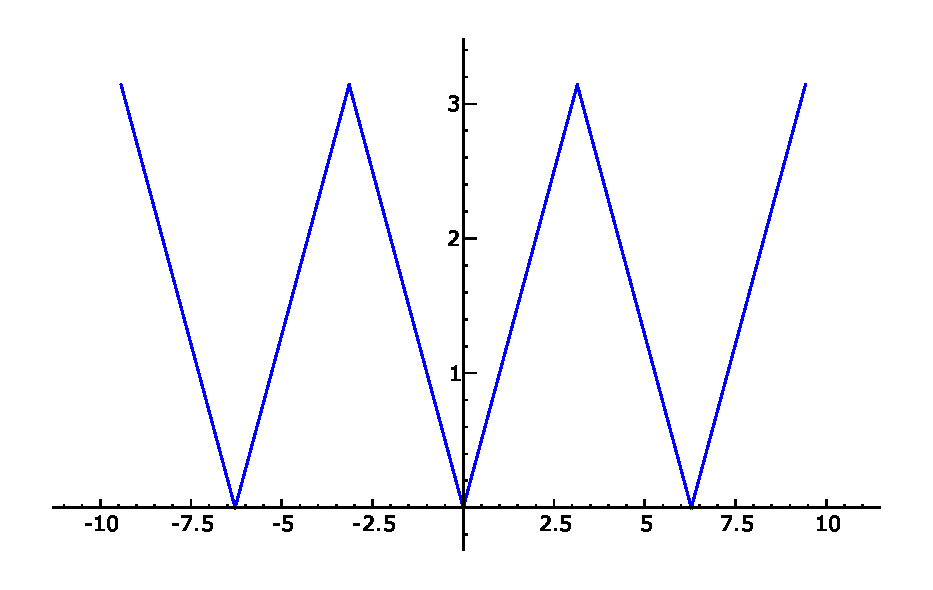
\includegraphics[width=\textwidth]{img/2April2008triangleWave.eps}
\end{center}
\caption{The Triangle Wave.}
\label{fig:2April2008:triangleWave}
\end{figure}
We can calculate its Fourier series simply by using the
$a_n$ and $b_n$ cofficients. Observe
\begin{subequations}
\begin{align}
a_{0} &= \frac{1}{\pi}\int^{\pi}_{-\pi}f(\theta)d\theta \\
&= \frac{1}{\pi}\left(\int^{\pi}_{0}\theta d\theta +
\int^{0}_{-\pi}-\theta d\theta\right) \\
&= \frac{2}{\pi}\int^{\pi}_{0}\theta d\theta \\
&= \frac{2}{\pi}\left(\frac{\theta^2}{2}\Big|^{\pi}_{0}\right)\\
&= \frac{2}{\pi}\left(\frac{\pi^2}{2}\right) \\
&= \pi
\end{align}
\end{subequations}
Also observe that
\begin{equation}
f(-\theta)=f(\theta)
\end{equation}
so the $b_{n}=0$ for all $n\in\mathbb{Z}$. The only
coefficients we have to calculate are the $a_{n}$. Observe
\begin{subequations}
\begin{align}
a_{n} &=
\frac{2}{\pi}\int^{\pi}_{0}\theta\cos(\theta)d\theta \\
&=\frac{\pi}{2}\left[\frac{\theta\sin(n\theta)}{n}\Big|^{\pi}_{0}-\int^{\pi}_{0}\frac{\sin(n\theta)}{n}d\theta\right]\\
&=\frac{2}{\pi}\left[\left(0\right)+\frac{\cos(n\theta)}{n^2}\Big|^{\pi}_{0}\right] \\
&= \frac{2}{\pi}\left(\frac{(-1)^{n}-1}{n^{2}}\right) \\
&= \begin{cases} 0\qquad \text{$n$ is even} \\
-4/(n^2\pi)\qquad\text{$n$ is odd} 
\end{cases}
\end{align}
\end{subequations}
Now we can plug these coefficients into the Fourier series
to find
\begin{subequations}\label{eq:2April2008:fourierSeriesAbsoluteTheta}
\begin{align}
f(\theta) &= \frac{a_0}{2} +
\sum^{\infty}_{n=1}a_{n}\cos(n\theta) \\
&= \frac{\pi}{2} - \frac{4}{\pi}\sum^{\infty}_{n=1}\frac{\cos((2n-1)\theta)}{(2n-1)^2}
\end{align}
\end{subequations}
Now that we have expanded it, the question becomes:
\emph{does the Fourier series converge?} The answer is
yes. We observe that $\cos(\theta)\leq 1$ and 
\begin{equation}
\frac{1}{(2n-1)^2}\leq\frac{1}{n^2}
\end{equation}
thus term for term we have the inequality
\begin{equation}
\sum^{\infty}_{n=1}\frac{\cos((2n-1)\theta)}{(2n-1)^2} \leq \sum^{\infty}_{n=1}\frac{1}{n^2}.
\end{equation}
We know that $\sum 1/n^2$ converges (for a handwavy argument
if one is unconvinced: $\sum 1/n^2 \leq \int^{\infty}_{1}
(1/n^2)dn <\infty$ so the sum is finite), and our Fourier
series is less than this convergent sum, so it must converge
(by the Weierstrass M-test). 

% lambda x: (pi/2) - (4/pi)*sum([cos((2*k-1)*x)/((2*k-1)^2) for k in range(1,10)])

\begin{figure}[h]
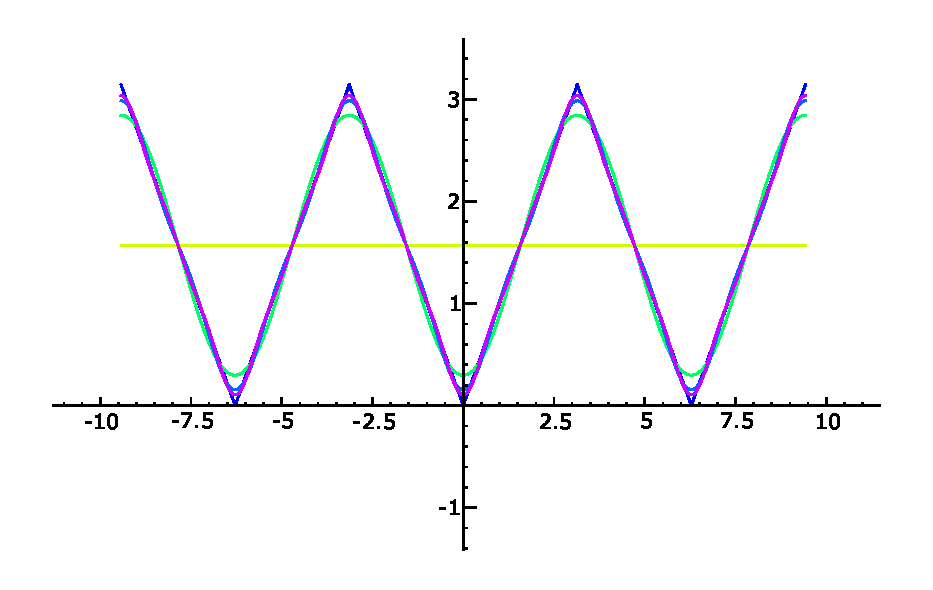
\includegraphics[width=\textwidth]{img/2April2008img2.eps}
\caption[Partial Sums of Fourier Expansion of Triangle Wave]{The Partial sum to the Triangle wave with 1 through 5 terms. The actual triangle wave is shown in blue.}
\label{fig:2April2008:triangleWavePartialSum}
\end{figure}



\end{ex}
